% EPC flow charts
% Author: Fabian Schuh
\documentclass{article}
\usepackage{myflowchart}

\begin{document}

\begin{tikzpicture}

\begin{scope}[node distance=5mm and 5mm]

\node [ item=2](a) at (1,1) {%
            \textbf{特色}
            \nodepart[text width = 8.2cm]{two}
            \begin{enumerate}
            	\item 使用LYX與SW,高度自動化產生django-compatible html(省下很多細微瑣碎步驟)。
            	\item 讓SW與LYX產生的網頁能夠正確顯示。如SW export links時有點問題,要記錄下可行步驟,並嘗試自動化。
           \end{enumerate}
            };

	\node [above right = of a, align = center, anchor = south] (title){
\includegraphics[width=0.12\textwidth]{../logos_creation/ancestor_veneration}};
	\node [right = of title,text height=1.5ex,text depth=.25ex,] {\Huge Plans};
	\node [left = of title,text height=1.5ex,text depth=.25ex,] {\Huge Website};
	%\parbox[c][][c]{3.2cm}{\Huge website}\parbox[c][][c]{0.15\textwidth}{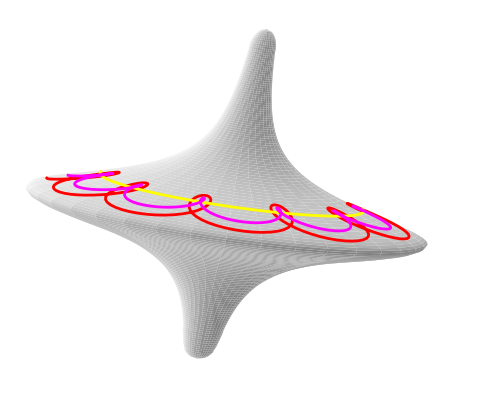
\includegraphics[width=0.15\textwidth]{../../figs/logo_June27_2016.png}}\parbox[c][][c]{3.6cm}{\Huge planning}};


\node [ item=2, below right = of title.south, anchor = north west](small) {%
            \textbf{unfinished}
            \nodepart[text width = 8.2cm]{two}
            \begin{enumerate}
            	\item look up collected volcab and write post.(四五月有不少還沒查的)
           \end{enumerate}
            };

\node [ wideitem=2, below right = of a, anchor = north](LYX) {%
            \textbf{creating posts utilizing LYX}
            \nodepart[text width = 16.5cm, align = left]{two}When generating html files from LYX for our website, a few steps need to be followed in order to make it work. Most webpages on this site are generated by LYX, even the django-compatible html pages. In order to make this work a few things has to be followed during the LYX exporting process. Five types of posts can be generated after running the function or button of LYX's HTML export:
            \begin{enumerate}
            	\item normal, nothing needs to be done.
            	\item 若有scribd pdf preview embeded code,打開LYX2HTML\_replace\_str.py確認裡面的檔名是你的檔案,然後python執行LYX2HTML\_replace\_str.py。To generate webpost that has Scribd pdf preview embed code, after LYX html export, run LYX2HTML\_str\_replace.py
		\item 若要加入本工作室設計的banner header(網頁上方的logo加標題加一條線),跑LYX2HTML\_banner\_replace.py。To generate webpost that has the head banner, after LYX html export, run LYX2HTML\_header\_replace.py
		\item 若有數學公式,在使用LYX html export之前,要去設定converter,加上-mathjax指令,用完之後記得要把converter的-mathjax指令移除,也就是設定回原本狀態。這步驟有點麻煩,如何改進?
		\item 若輸出的html檔包含有需要被伺服的圖檔,則LYX插入圖片時可按照以下整理好的流程
		\begin{enumerate}
			\item 將所需圖片先複製到與LYX檔案相同位置(在myblogpost資料夾那邊,不是template那邊),名為static的資料夾下。
			\item 在LYX檔中從上述資料夾插入圖片
			\item 執行LYX html export功能,此功能經過我們更改,檔案會自動export至template資料夾。這樣圖片也會copy到那邊的static資料夾。
			\item 運行django指令collectstatic收集所有template資料夾中要被伺服的眾多static資料夾。
			\item (若有信心沒有bug可省略)設定debug=true(這樣本地端static資料夾才會被伺服),運行django本地端測試local test server。沒問題設定回debug=false。
			\item git commit時記得要track圖片!!!git push to deploy.
		\end{enumerate}
           \end{enumerate}
            };
\node [ wideitem=2, below = of LYX, anchor = north](SW) {%
            \textbf{creating posts utilizing SW}
            \nodepart[text width = 16.5cm, align = left]{two}Have to write this down before I forget.
            \begin{enumerate}
            	\item 目前是使用SW的export html指令後,用vim打開,手動移除所有mdframe的<>區域。mdframe區域是要產生pdf時所使用的。SW編輯時的html code tex insert才是產生html listing envr網頁版程式區域。
		\begin{enumerate}
			\item 可執行一vim script移除所有<spam mdframe><spame>及其中所有內容。
			\item 或執行python達到相同動作。
		\end{enumerate}
           \end{enumerate}
            };

\end{scope}
\end{tikzpicture}
\end{document}
